\section{The Fast Multipole Method}

\begin{frame}{A tree of boxes, neighbors and interaction lists}
  \begin{itemize}
      \item Divide the square $\Omega$ into $4^L$ equisized smaller boxes
      \vspace{4mm}
      \item Given a box $\tau$ :\\
          - The parent of $\tau$ is the box on the following higher level that contains $\tau$\\
          - The children of $\tau$ compose the set of boxes with $\tau$ as their parent\\
          - The neighbors of $\tau$ compose the set of boxes that directly touch $\tau$\\
          - The interaction list of $\tau$ is the set of all boxes $\sigma$ such that $\sigma$ and $\tau$ are on the same level, and do not touch each other, but their parents touch each other.\\
  \end{itemize}
    \vspace{4mm}
  \begin{figure}[htp]
      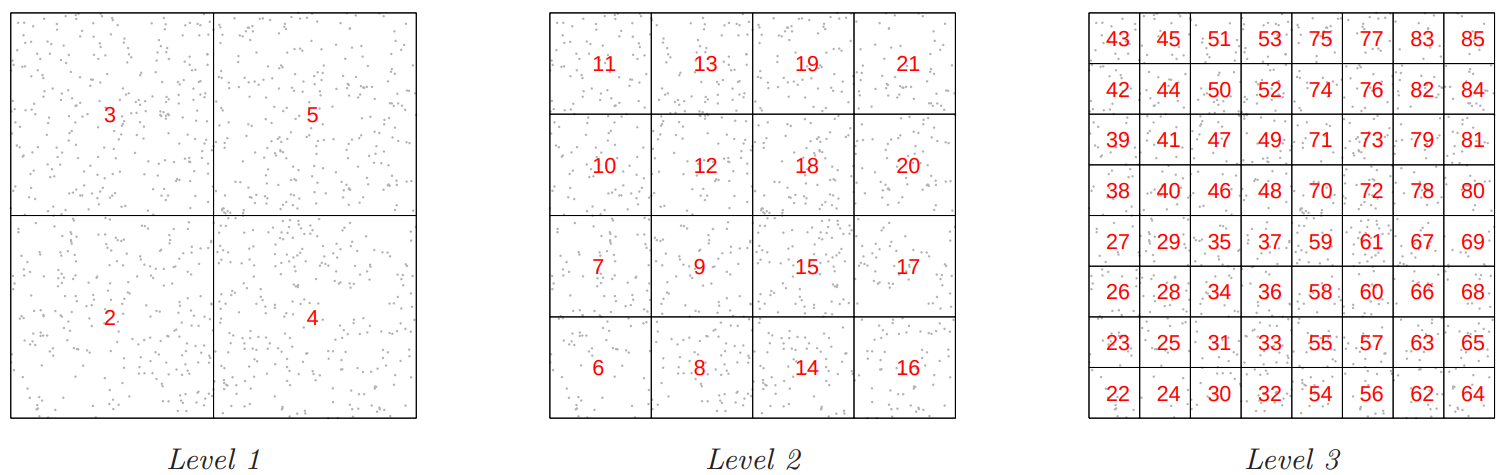
\includegraphics[width=21cm]{presentation/img/tree_of_boxes.png}
      \label{fig:particles}
  \end{figure}

\end{frame}


\begin{frame}{The Algorithm}
  1. Construct the tree and all interaction lists\\
  \vspace{3mm}
  2. Compute: $\hat{\mathbf{q}}^{\tau}=\mathbf{T}_{\tau}^{\mathrm{ofs}} \mathbf{q}\left(I_{\tau}\right)$\\
    \vspace{4mm}
  \begin{figure}[htp]
      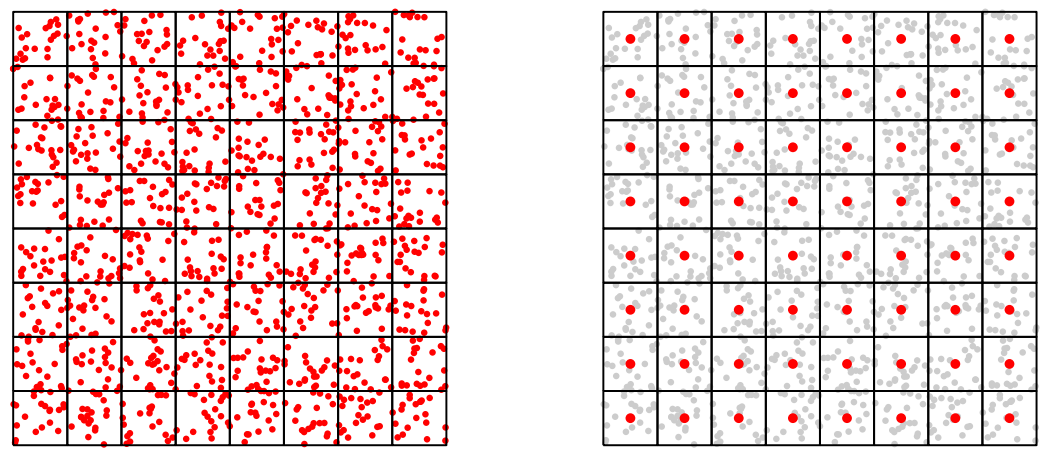
\includegraphics[width=21cm]{presentation/img/outgoing1.png}
      \label{fig:particles}
  \end{figure}
\end{frame}

\begin{frame}{The Algorithm}
  1. Construct the tree and all interaction lists\\
  \vspace{3mm}
  2. Compute: $\hat{\mathbf{q}}^{\tau}=\mathbf{T}_{\tau}^{\mathrm{ofs}} \mathbf{q}\left(I_{\tau}\right)$\\
  \vspace{8mm}
  \setlength{\parindent}{4ex}  $\rightarrow$ the outgoing-from-source translation operator results from truncating \\ \setlength{\parindent}{4ex} the outgoing expansion of $\Omega$ to order P
       \begin{equation}
          \begin{split}
            q_0 &= \sum_j^N m_j \\
            q_k &= - \sum_j^N \frac{m_j}{k} (\vct y - \vct c_\sigma)^k
          \end{split}
        \end{equation}
\end{frame}


 \begin{frame}{The Algorithm}
  1. Construct the tree and all interaction lists\\
  \vspace{3mm}
  2. Compute: $\hat{\mathbf{q}}^{\tau}=\mathbf{T}_{\tau}^{\mathrm{ofs}} \mathbf{q}\left(I_{\tau}\right)$\\
  \vspace{3mm}
  3. Compute: $\hat{\mathbf{q}}^{\tau}=\sum_{\sigma \in \mathcal{L}_{\tau}^{\text {child }}} \mathrm{T}_{\tau, \sigma}^{\text {ofo }} \hat{\mathbf{q}}^{\sigma}$\\

  \vspace{6mm}
  \begin{figure}[!tbp]
    \centering
    \begin{minipage}[b]{0.3\textwidth}
      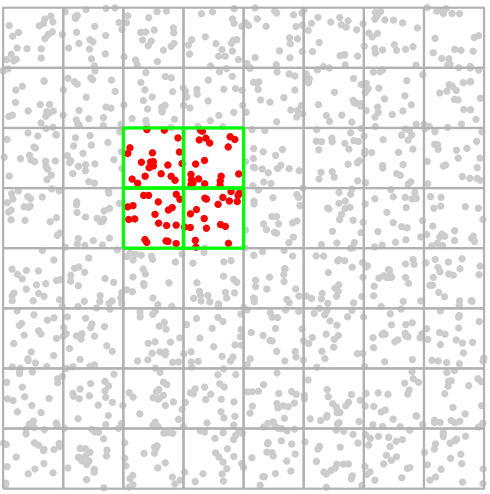
\includegraphics[width=\textwidth]{dot_magenta}
    \end{minipage}
    \hfill
    \begin{minipage}[b]{0.3\textwidth}
      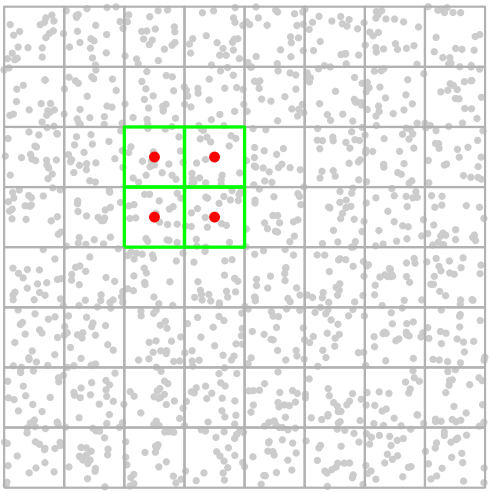
\includegraphics[width=\textwidth]{dot_magenta1}
    \end{minipage}
    \hfill
    \begin{minipage}[b]{0.3\textwidth}
      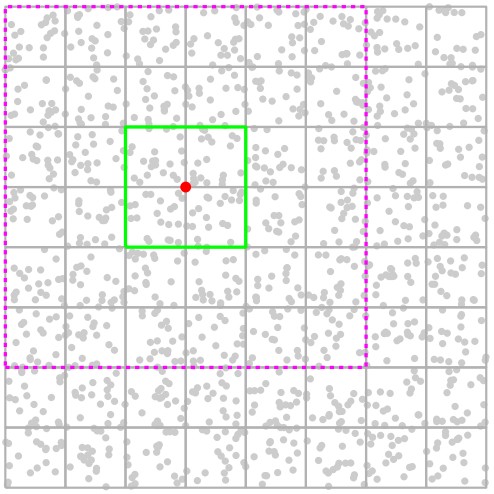
\includegraphics[width=\textwidth]{dot_magenta2}
    \end{minipage}
  \end{figure}

\end{frame}


 \begin{frame}{The Algorithm}
  1. Construct the tree and all interaction lists\\
  \vspace{3mm}
  2. Compute: $\hat{\mathbf{q}}^{\tau}=\mathbf{T}_{\tau}^{\mathrm{ofs}} \mathbf{q}\left(I_{\tau}\right)$\\
  \vspace{3mm}
  3. Compute: $\hat{\mathbf{q}}^{\tau}=\sum_{\sigma \in \mathcal{L}_{\tau}^{\text {child }}} \mathrm{T}_{\tau, \sigma}^{\text {ofo }} \hat{\mathbf{q}}^{\sigma}$\\

  \vspace{6mm}
  \begin{figure}[!tbp]
    \centering
    \begin{minipage}[b]{0.3\textwidth}
      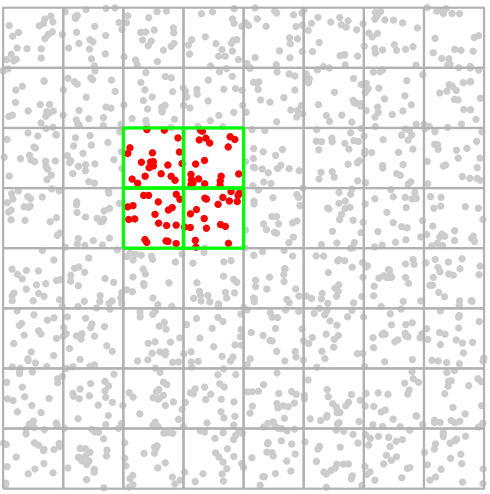
\includegraphics[width=\textwidth]{dot_magenta}
    \end{minipage}
    \hfill
    \begin{minipage}[b]{0.3\textwidth}
      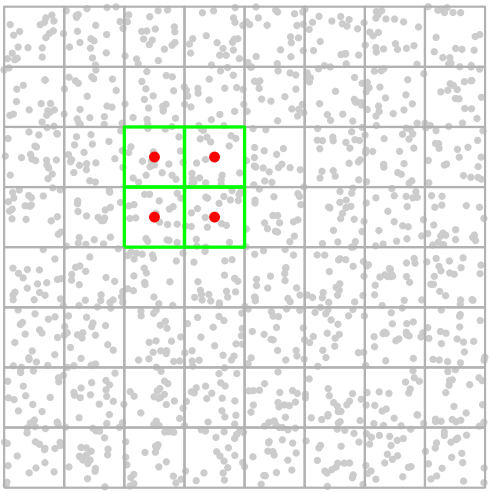
\includegraphics[width=\textwidth]{dot_magenta1}
    \end{minipage}
    \hfill
    \begin{minipage}[b]{0.3\textwidth}
      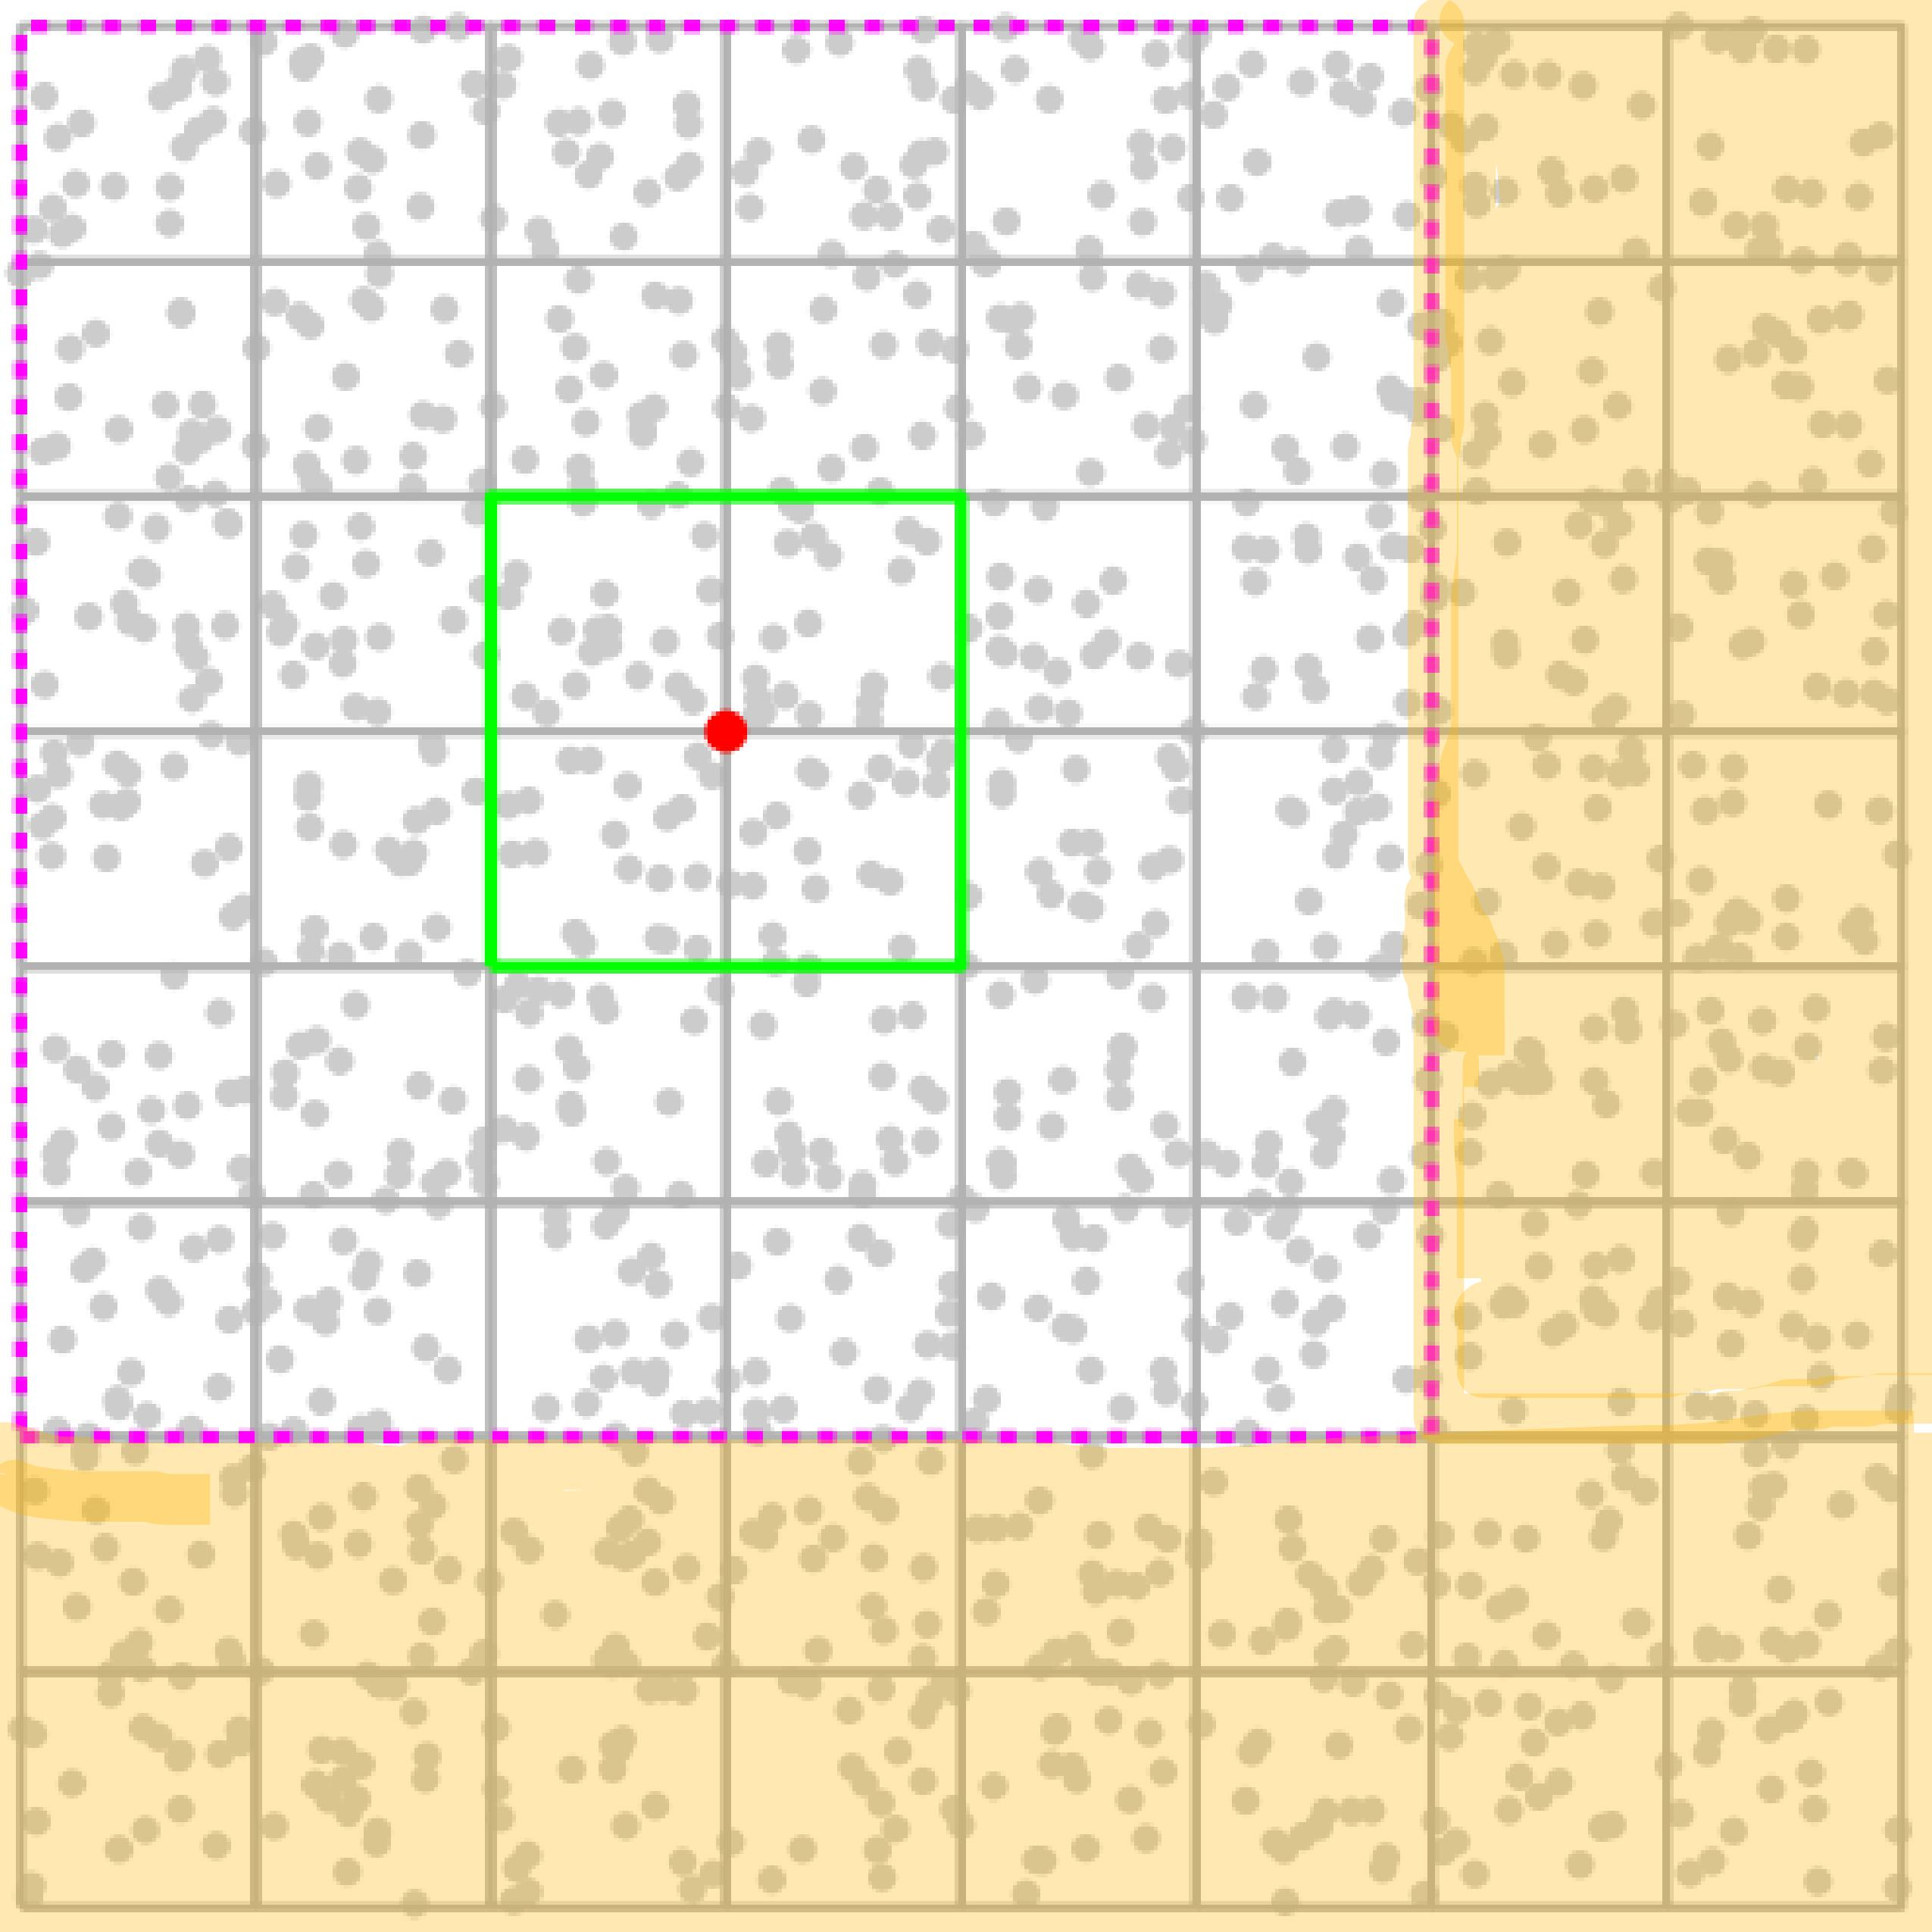
\includegraphics[width=\textwidth]{presentation/img/magenta_yellow1.jpg}
    \end{minipage}
  \end{figure}

\end{frame}

 \begin{frame}{The Algorithm}
  1. Construct the tree and all interaction lists\\
  \vspace{3mm}
  2. Compute: $\hat{\mathbf{q}}^{\tau}=\mathbf{T}_{\tau}^{\mathrm{ofs}} \mathbf{q}\left(I_{\tau}\right)$\\
  \vspace{3mm}
  3. Compute: $\hat{\mathbf{q}}^{\tau}=\sum_{\sigma \in \mathcal{L}_{\tau}^{\text {child }}} \mathrm{T}_{\tau, \sigma}^{\text {ofo }} \hat{\mathbf{q}}^{\sigma}$\\

  \vspace{6mm}
  \begin{figure}[!tbp]
    \centering
    \begin{minipage}[b]{0.3\textwidth}
      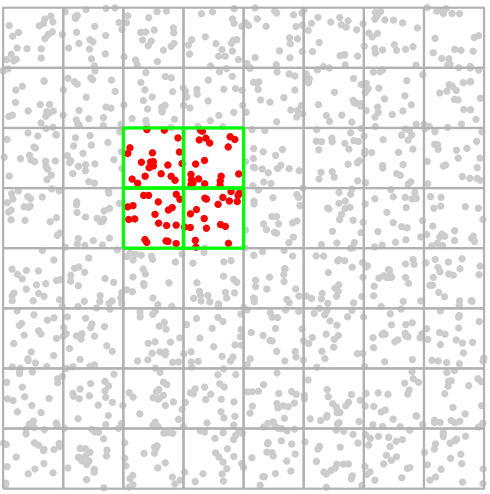
\includegraphics[width=\textwidth]{dot_magenta}
    \end{minipage}
    \hfill
    \begin{minipage}[b]{0.3\textwidth}
      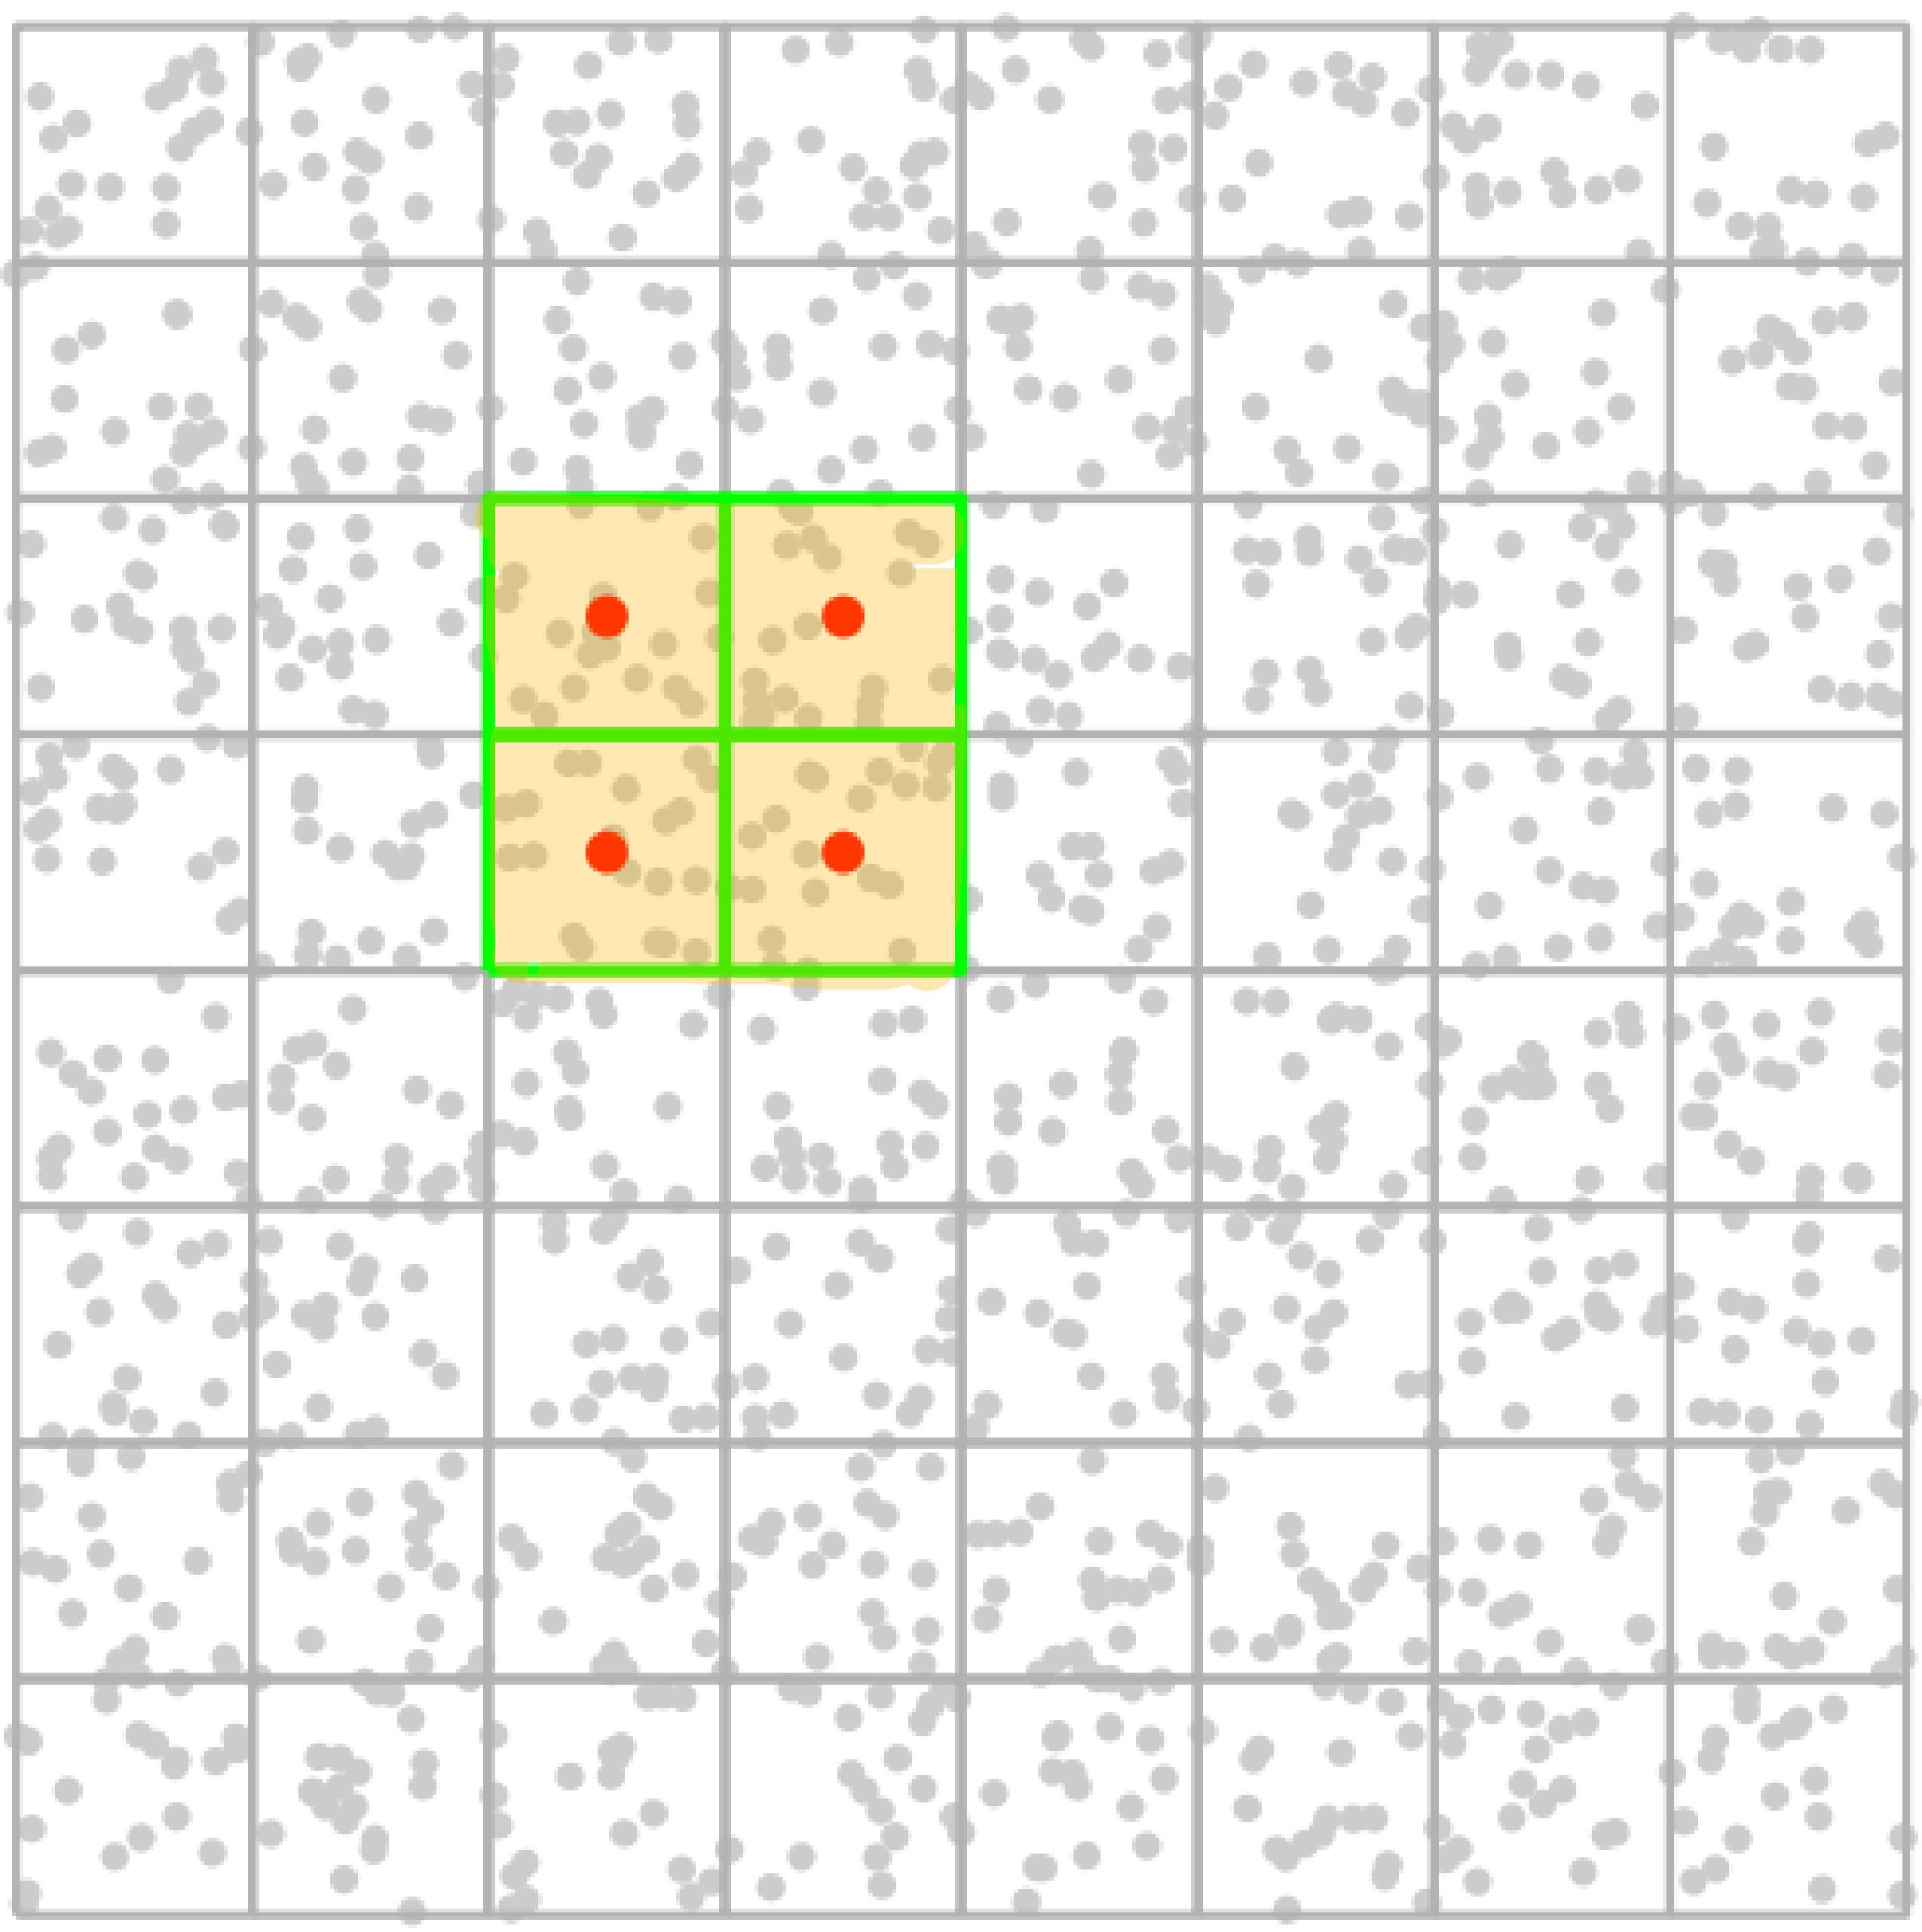
\includegraphics[width=\textwidth]{presentation/img/magenta_yeallow2.jpg}
    \end{minipage}
    \hfill
    \begin{minipage}[b]{0.3\textwidth}
      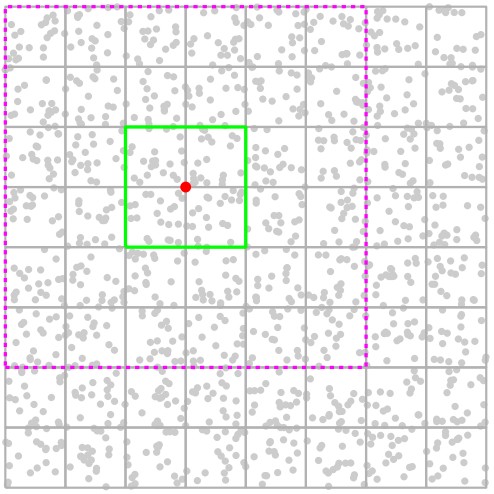
\includegraphics[width=\textwidth]{dot_magenta2}
    \end{minipage}
  \end{figure}

\end{frame}


  \begin{frame}{The Algorithm}
  1. Construct the tree and all interaction lists\\
  \vspace{3mm}
  2. Compute: $\hat{\mathbf{q}}^{\tau}=\mathbf{T}_{\tau}^{\mathrm{ofs}} \mathbf{q}\left(I_{\tau}\right)$\\
  \vspace{3mm}
  3. Compute: $\hat{\mathbf{q}}^{\tau}=\sum_{\sigma \in \mathcal{L}_{\tau}^{\text {child }}} \mathrm{T}_{\tau, \sigma}^{\text {ofo }} \hat{\mathbf{q}}^{\sigma}$\\

  \vspace{8mm}
  \setlength{\parindent}{4ex}  $\rightarrow$ The outgoing-from-outgoing translation operator $T_{\tau, \sigma}^{o f o}$ can be \\
  \setlength{\parindent}{4ex}  derived from truncating the series to the first $\mathrm{P}$ terms:

  \begin{figure}[!tbp]
    \centering
    \begin{minipage}[b]{0.3\textwidth}
        \begin{array}{l}
          \hat{q}_{0}^{\tau}=\hat{q}_{0}^{\sigma} \\
          \hat{q}_{i}^{\tau}=-\hat{q}_{0}^{\sigma} \frac{1}{i}\left(c_{\sigma}-c_{\tau}\right)^{i}+\sum_{j=1}^{i} \hat{q}_{j}^{\sigma}\left(\begin{array}{c}
          i-1 \\
          j-1
          \end{array}\right)\left(c_{\sigma}-c_{\tau}\right)^{i-j}
          \end{array}
    \end{minipage}
    \hfill
    \begin{minipage}[b]{0.3\textwidth}
      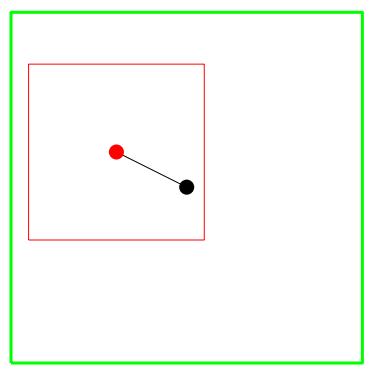
\includegraphics[width=5cm]{presentation/img/ofo.png}
    \end{minipage}
  \end{figure}

\end{frame}

\begin{frame}{The Algorithm}
  1. Construct the tree and all interaction lists\\
  \vspace{3mm}
  2. Compute: $\hat{\mathbf{q}}^{\tau}=\mathbf{T}_{\tau}^{\mathrm{ofs}} \mathbf{q}\left(I_{\tau}\right)$\\
  \vspace{3mm}
  3. Compute: $\hat{\mathbf{q}}^{\tau}=\sum_{\sigma \in \mathcal{L}_{\tau}^{\text {child }}} \mathrm{T}_{\tau, \sigma}^{\text {ofo }} \hat{\mathbf{q}}^{\sigma}$\\
  \vspace{3mm}
  4. Compute: $\hat{\mathbf{u}}^{\tau}=\hat{\mathbf{u}}^{\tau}+\mathrm{T}_{\tau, \sigma}^{\mathrm{ifi}} \hat{\mathbf{u}}^{\sigma} \text { and } \quad \hat{\boldsymbol{u}}^{\tau}=\hat{\boldsymbol{u}}^{\tau}+\sum_{\sigma \in L_{\tau}^{i n t}} T_{\tau, \sigma}^{i f o} \widehat{\boldsymbol{q}}^{\sigma}$\\
  \vspace{3mm}
  \begin{figure}[!tbp]
    \centering
    \begin{minipage}[b]{0.35\textwidth}
      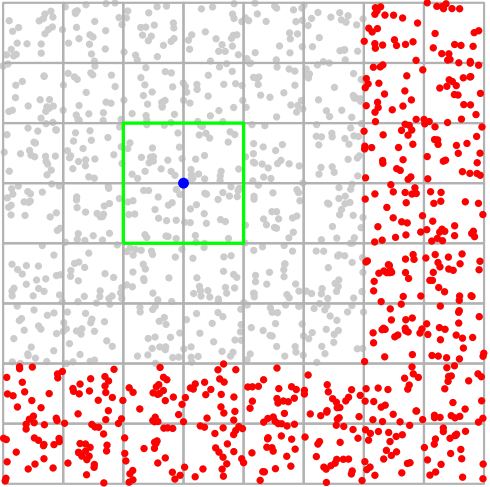
\includegraphics[width=\textwidth]{dot_magenta3}
    \end{minipage}
    \hfill
    \begin{minipage}[b]{0.35\textwidth}
      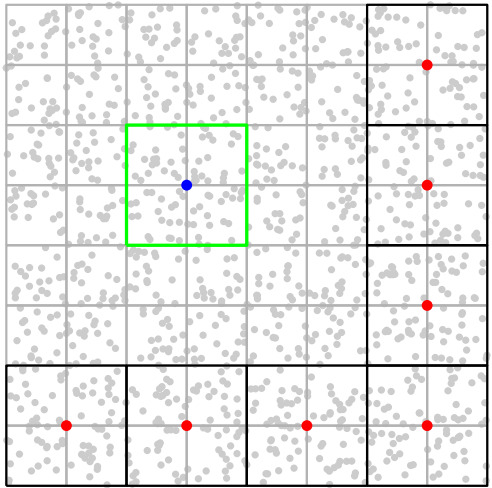
\includegraphics[width=\textwidth]{dot_magenta4}
    \end{minipage}
  \end{figure}
\end{frame}

\begin{frame}{The Algorithm}
  1. Construct the tree and all interaction lists\\
  \vspace{3mm}
  2. Compute: $\hat{\mathbf{q}}^{\tau}=\mathbf{T}_{\tau}^{\mathrm{ofs}} \mathbf{q}\left(I_{\tau}\right)$\\
  \vspace{3mm}
  3. Compute: $\hat{\mathbf{q}}^{\tau}=\sum_{\sigma \in \mathcal{L}_{\tau}^{\text {child }}} \mathrm{T}_{\tau, \sigma}^{\text {ofo }} \hat{\mathbf{q}}^{\sigma}$\\
  \vspace{3mm}
  4. Compute: $\hat{\mathbf{u}}^{\tau}=\hat{\mathbf{u}}^{\tau}+\mathrm{T}_{\tau, \sigma}^{\mathrm{ifi}} \hat{\mathbf{u}}^{\sigma} \text { and } \quad \hat{\boldsymbol{u}}^{\tau}=\hat{\boldsymbol{u}}^{\tau}+\sum_{\sigma \in L_{\tau}^{i n t}} T_{\tau, \sigma}^{i f o} \widehat{\boldsymbol{q}}^{\sigma}$\\
  \vspace{3mm}
  \begin{figure}[!tbp]
    \centering
    \begin{minipage}[b]{0.35\textwidth}
      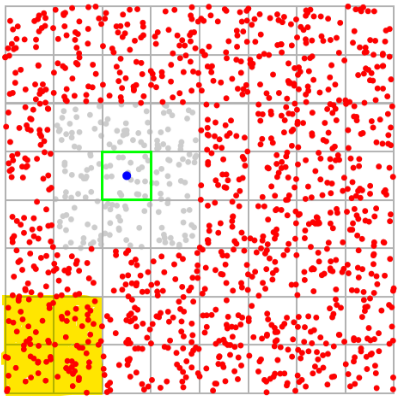
\includegraphics[width=\textwidth]{dot_magenta5}
    \end{minipage}
    \hfill
    \begin{minipage}[b]{0.35\textwidth}
      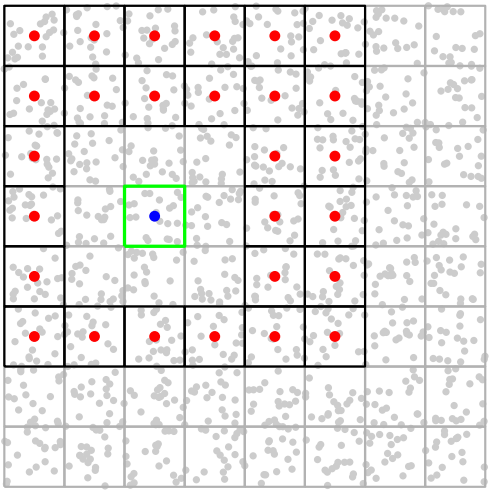
\includegraphics[width=\textwidth]{dot_magenta6}
    \end{minipage}
  \end{figure}
\end{frame}


\begin{frame}{The Algorithm}
  1. Construct the tree and all interaction lists\\
  \vspace{3mm}
  2. Compute: $\hat{\mathbf{q}}^{\tau}=\mathbf{T}_{\tau}^{\mathrm{ofs}} \mathbf{q}\left(I_{\tau}\right)$\\
  \vspace{3mm}
  3. Compute: $\hat{\mathbf{q}}^{\tau}=\sum_{\sigma \in \mathcal{L}_{\tau}^{\text {child }}} \mathrm{T}_{\tau, \sigma}^{\text {ofo }} \hat{\mathbf{q}}^{\sigma}$\\
  \vspace{3mm}
  4. Compute: $\hat{\mathbf{u}}^{\tau}=\hat{\mathbf{u}}^{\tau}+\mathrm{T}_{\tau, \sigma}^{\mathrm{ifi}} \hat{\mathbf{u}}^{\sigma} \text { and } \quad \hat{\boldsymbol{u}}^{\tau}=\hat{\boldsymbol{u}}^{\tau}+\sum_{\sigma \in L_{\tau}^{i n t}} T_{\tau, \sigma}^{i f o} \widehat{\boldsymbol{q}}^{\sigma}$\\
  \vspace{8mm}
  \setlength{\parindent}{4ex}  $\rightarrow$ The incoming-from-incoming translation operator results\\ \setlength{\parindent}{4ex} from truncating the series to the first $P$ terms:
  $$
  \hat{u}_{i}^{\sigma}=\sum_{j=i}^{\infty} \hat{u}_{j}^{\tau}\left(\begin{array}{l}
  j \\
  i
  \end{array}\right)\left(\boldsymbol{c}_{\sigma}-\boldsymbol{c}_{\tau}\right)^{j-i}
  $$\\

  
\end{frame}

\begin{frame}{The Algorithm}
  1. Construct the tree and all interaction lists\\
  \vspace{3mm}
  2. Compute: $\hat{\mathbf{q}}^{\tau}=\mathbf{T}_{\tau}^{\mathrm{ofs}} \mathbf{q}\left(I_{\tau}\right)$\\
  \vspace{3mm}
  3. Compute: $\hat{\mathbf{q}}^{\tau}=\sum_{\sigma \in \mathcal{L}_{\tau}^{\text {child }}} \mathrm{T}_{\tau, \sigma}^{\text {ofo }} \hat{\mathbf{q}}^{\sigma}$\\
  \vspace{3mm}
  4. Compute: $\hat{\mathbf{u}}^{\tau}=\hat{\mathbf{u}}^{\tau}+\mathrm{T}_{\tau, \sigma}^{\mathrm{ifi}} \hat{\mathbf{u}}^{\sigma} \text { and } \quad \hat{\boldsymbol{u}}^{\tau}=\hat{\boldsymbol{u}}^{\tau}+\sum_{\sigma \in L_{\tau}^{i n t}} T_{\tau, \sigma}^{i f o} \widehat{\boldsymbol{q}}^{\sigma}$\\
  \vspace{8mm}
  \setlength{\parindent}{4ex}  $\rightarrow$ The incoming-from-outgoing translation operator results\\ \setlength{\parindent}{4ex} from truncating the incoming expansion to the first $P$ terms:
    \begin{equation}
      \begin{split}
        u_0 &= q_0 \log(\vct c_\tau - \vct c_\sigma) + \sum_{j=1}^\infty q_j (-1)^j \frac 1 {(\vct c_\sigma - \vct c_\tau)^j} \\
        u_k &= -q_0 \frac 1 {k(\vct c_\sigma - \vct c_\tau)^k} + \sum_{j=1}^\infty q_j (-1)^j \mat{k+j-1\\j-1} \frac 1 {(\vct c_\sigma - \vct c_\tau)^{k+j}} \\
      \end{split}
    \end{equation}
\end{frame}


  \begin{frame}{The Algorithm}
  1. Construct the tree and all interaction lists\\
  \vspace{3mm}
  2. Compute: $\hat{\mathbf{q}}^{\tau}=\mathbf{T}_{\tau}^{\mathrm{ofs}} \mathbf{q}\left(I_{\tau}\right)$\\
  \vspace{3mm}
  3. Compute: $\hat{\mathbf{q}}^{\tau}=\sum_{\sigma \in \mathcal{L}_{\tau}^{\text {child }}} \mathrm{T}_{\tau, \sigma}^{\text {ofo }} \hat{\mathbf{q}}^{\sigma}$\\
  \vspace{3mm}
  4. Compute: $\hat{\mathbf{u}}^{\tau}=\hat{\mathbf{u}}^{\tau}+\mathrm{T}_{\tau, \sigma}^{\mathrm{ifi}} \hat{\mathbf{u}}^{\sigma} \text { and } \quad \hat{\boldsymbol{u}}^{\tau}=\hat{\boldsymbol{u}}^{\tau}+\sum_{\sigma \in L_{\tau}^{i n t}} T_{\tau, \sigma}^{i f o} \widehat{\boldsymbol{q}}^{\sigma}$\\
  \vspace{3mm}
  5. Compute:$\mathbf{u}\left(I_{\tau}\right)=\mathbf{T}_{\tau}^{\mathrm{tfi}}\hat{\mathbf{u}}^{\tau}+\mathbf{A}\left(I_{\tau}, I_{\tau}\right) \mathbf{q}\left(I_{\tau}\right)+\sum_{\sigma \in \mathcal{L}_{\tau}^{\mathrm{nei}}} \mathbf{A}\left(I_{\tau}, I_{\sigma}\right) \mathbf{q}\left(I_{\sigma}\right)$\\
  \vspace{3mm}
  \begin{figure}[htp]
      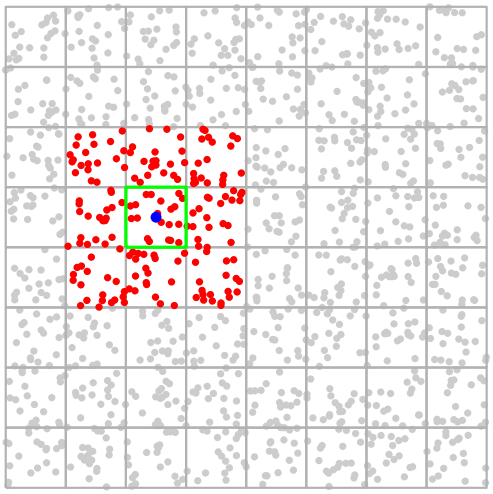
\includegraphics[width=7cm]{dot_magenta7}
      \label{fig:particles}
  \end{figure}

\end{frame}

  \begin{frame}{The Algorithm}
  1. Construct the tree and all interaction lists\\
  \vspace{3mm}
  2. Compute: $\hat{\mathbf{q}}^{\tau}=\mathbf{T}_{\tau}^{\mathrm{ofs}} \mathbf{q}\left(I_{\tau}\right)$\\
  \vspace{3mm}
  3. Compute: $\hat{\mathbf{q}}^{\tau}=\sum_{\sigma \in \mathcal{L}_{\tau}^{\text {child }}} \mathrm{T}_{\tau, \sigma}^{\text {ofo }} \hat{\mathbf{q}}^{\sigma}$\\
  \vspace{3mm}
  4. Compute: $\hat{\mathbf{u}}^{\tau}=\hat{\mathbf{u}}^{\tau}+\mathrm{T}_{\tau, \sigma}^{\mathrm{ifi}} \hat{\mathbf{u}}^{\sigma} \text { and } \quad \hat{\boldsymbol{u}}^{\tau}=\hat{\boldsymbol{u}}^{\tau}+\sum_{\sigma \in L_{\tau}^{i n t}} T_{\tau, \sigma}^{i f o} \widehat{\boldsymbol{q}}^{\sigma}$\\
  \vspace{3mm}
  5. Compute:$\mathbf{u}\left(I_{\tau}\right)=\mathbf{T}_{\tau}^{\mathrm{tfi}}\hat{\mathbf{u}}^{\tau}+\mathbf{A}\left(I_{\tau}, I_{\tau}\right) \mathbf{q}\left(I_{\tau}\right)+\sum_{\sigma \in \mathcal{L}_{\tau}^{\mathrm{nei}}} \mathbf{A}\left(I_{\tau}, I_{\sigma}\right) \mathbf{q}\left(I_{\sigma}\right)$\\
  \vspace{3mm}
  \begin{figure}[htp]
      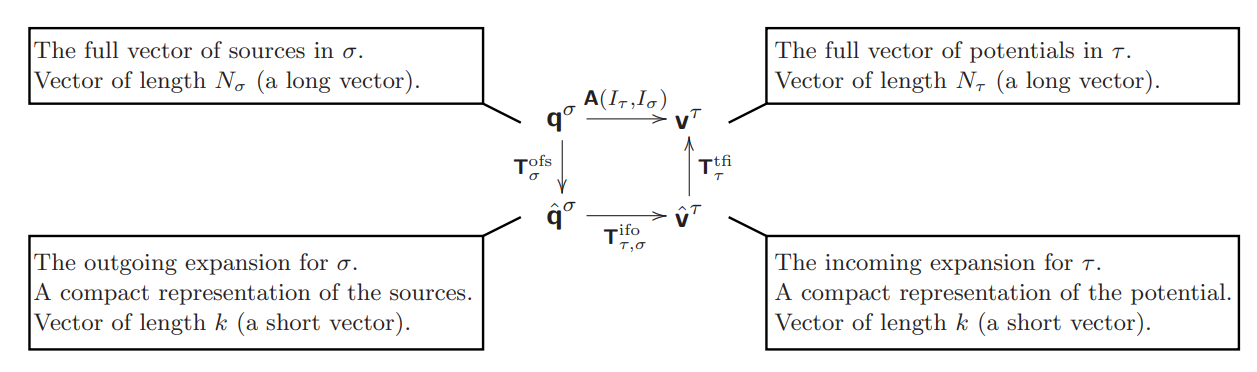
\includegraphics[width=22cm]{presentation/img/A_explanation.png}
      \label{fig:particles}
  \end{figure}

\end{frame}

\begin{frame}{The Algorithm}
  1. Construct the tree and all interaction lists\\
  \vspace{3mm}
  2. Compute: $\hat{\mathbf{q}}^{\tau}=\mathbf{T}_{\tau}^{\mathrm{ofs}} \mathbf{q}\left(I_{\tau}\right)$\\
  \vspace{3mm}
  3. Compute: $\hat{\mathbf{q}}^{\tau}=\sum_{\sigma \in \mathcal{L}_{\tau}^{\text {child }}} \mathrm{T}_{\tau, \sigma}^{\text {ofo }} \hat{\mathbf{q}}^{\sigma}$\\
  \vspace{3mm}
  4. Compute: $\hat{\mathbf{u}}^{\tau}=\hat{\mathbf{u}}^{\tau}+\mathrm{T}_{\tau, \sigma}^{\mathrm{ifi}} \hat{\mathbf{u}}^{\sigma} \text { and } \quad \hat{\boldsymbol{u}}^{\tau}=\hat{\boldsymbol{u}}^{\tau}+\sum_{\sigma \in L_{\tau}^{i n t}} T_{\tau, \sigma}^{i f o} \widehat{\boldsymbol{q}}^{\sigma}$\\
  \vspace{3mm}
  5. Compute:$\mathbf{u}\left(I_{\tau}\right)=\mathbf{T}_{\tau}^{\mathrm{tfi}}\hat{\mathbf{u}}^{\tau}+\mathbf{A}\left(I_{\tau}, I_{\tau}\right) \mathbf{q}\left(I_{\tau}\right)+\sum_{\sigma \in \mathcal{L}_{\tau}^{\mathrm{nei}}} \mathbf{A}\left(I_{\tau}, I_{\sigma}\right) \mathbf{q}\left(I_{\sigma}\right)$\\
\end{frame}

\begin{frame}{Error Analysis}
  \begin{itemize}
      \item All expansions have been reduced to P terms $\implies$ the potentials estimated by the FMM are not precise \\
       \vspace{3mm}
      \item The global error is similar to the worst-case local truncation error\\
       \vspace{3mm}
      \item It scales as $\alpha ^ \mathrm{P}$ where alpha $=\sqrt{2} /(4-\sqrt{2}) \approx 0.5469$\\
       \vspace{3mm}
      \item  $\implies$ To achieve a given tolerance $\varepsilon$, $\mathrm{P} \approx \log (\varepsilon) / \log (\alpha)$\\
       \vspace{3mm}
      \item If we assume that each leaf holds $\mathrm{O}(\mathrm{P})$ sources, then increasing P means that the asymptotic complexity of the 2D FMM is $\mathrm{O}(\mathrm{P} \mathrm{N})$. \\
       \vspace{3mm}
      \item $\implies$  As a result, the overall complexity scales as $\log (1 / \varepsilon) \mathrm{N}$ as $\varepsilon \rightarrow 0$ and $\mathrm{N} \rightarrow \infty$.
  \end{itemize}
\end{frame}
